\documentclass[8.01x]{subfiles}
\begin{document}

\chapter{Week 6: Homework 5}

\section{Problem 1: Geosynchronous orbit}

A satellite with a mass of $m_s = \SI{3e3}{kg}$ is in a planet's equatorial plane in a circular ``synchronous'' orbit. This means that an observer at the equator will see the satellite being stationary overhead (see figure below). The planet has mass $m_p = \SI{5.16e25}{kg}$ and a day of length $T = 0.7$ earth days (1 earth day = 24 hours).

\begin{center}
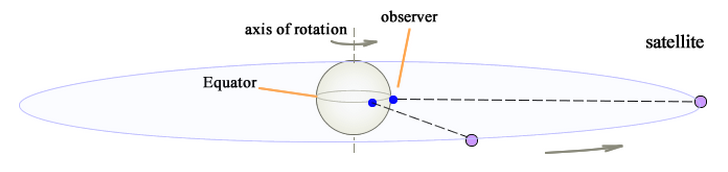
\includegraphics[scale=0.6]{Graphics/h5p1}
\end{center}

(a) How far from the center (in m) of the planet is the satellite?\\
(b) What is the escape velocity (in km/sec) of any object that is at the same distance from the center of the planet that you calculated in (a)?''

The day's length is $0.7 \cdot 24$ hours = 16.8 hours, or 60480 seconds. This must then be the orbital period of the satellite, since it is supposed to remain over the same point at all times.\\
I don't recall the exact formulas we learned from lecture (and if I did, I likely wouldn't a year from now), but I do remember that the total mechanical energy is exactly $\frac{1}{2} U$. The mechanical energy is then the sum of the current kinetic energy, and the gravitational potential energy:

\begin{align}
\frac{1}{2} \left(-\frac{G m_p m_s}{r}\right) &= \frac{1}{2} m_s v_{orb}^2 - \frac{G m_p m_s}{r}\\
\frac{G m_p m_s}{r} &= m_s v_{orb}^2\\
\frac{1}{r} &= \frac{v_{orb}^2}{G m_p}\\
r &= \frac{G m_p}{v_{orb}^2}
\end{align}

We can then write $v_{orb}$, the tangential velocity of the satellite, in terms of $r$ and $T$:

\begin{align}
v_{orb} &= \frac{2 \pi r}{T}\\
v_{orb}^2 &= \frac{4 \pi^2 r^2}{T^2}
\end{align}

Substitute into $r$ (by multiplying by the reciprocal, instead of having a 3-layer fraction):

\begin{align}
r &= G m_p \cdot \frac{T^2}{4 \pi^2 r^2}\\
r^3 &= \frac{G m_p T^2}{4 \pi^2}\\
r &= \left(\frac{G m_p T^2}{4 \pi^2}\right)^{1/3}
\end{align}

Next, part (b): what is the escape velocity at this distance $r$ from the planet?\\
I could re-derive the expression for the escape velocity as well, which wasn't that hard, but I recall that $v_{esc} = \sqrt{2} \times v_{orb}$, and we already have an expression for $v_{orb}$. Multiplying $v_{orb}$ by $\sqrt{2}$ and then simplifying:

\begin{align}
v_{orb} &= \frac{2 \pi}{T} \left(\frac{G m_p T^2}{4 \pi^2}\right)^{1/3}\\
v_{esc} &= \sqrt{2} \left(\frac{2 \pi G m_p}{T}\right)^{1/3}
\end{align}

However, they want the answer in \emph{km/sec}, so we need to divide that by 1000.

\section{Problem 2: Bungee jumper}

``A bungee jumper jumps (with no initial speed) from a tall bridge attached to a light elastic cord (bungee cord) of unstretched length $L$. The cord first straightens and then extends as the jumper falls. This prevents her from hitting the water! Suppose that the bungee cord behaves like a spring with spring constant $k = \SI{90}{N/m}$. The bridge is $h = \SI{100}{m}$ high and the jumper's mass is $m = \SI{65}{kg}$. Use $g = \SI{10}{m/s^2}$.

\begin{center}
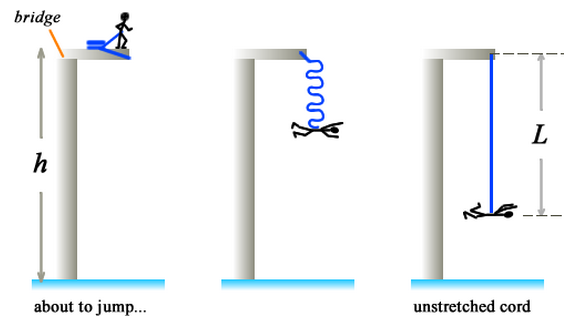
\includegraphics[scale=0.6]{Graphics/h5p2}
\end{center}

(a) What is the maximum allowed length L of the unstretched bungee cord (in m) to keep the jumper alive? (Assume that the spring constant doesn't depend on L).\\
(b) Before jumping, our jumper verified the spring constant of the cord. She lowered herself very slowly from the bridge to the full extent of the cord and when she is at rest she measured the distance to the water surface. What was the measured distance (in m)?''

Hitting the water at, say, 0.1 m/s will surely not be lethal, but I assume the condition is that she doesn't touch the water whatsoever, or we can't find an exact answer to the question.

I will use a coordinate system where $y$ increases downwards, and is centered on the bridge; thus the water is at $y = h$.\\
Also, I will use conservation of energy to solve this problem. My first solution was to find the total energy at $y = L$, after a period of free fall, and then the total energy at $y = h$, solving for $L$ that way. I realized later, reading the forums, that this is unnecessarily complex, so my much simpler solution is below.

The kinetic energy is zero both just as you jump (since it is done with zero speed) and as you almost reach the water: the velocity vector reverses at that point, so $v = 0$ at the lowest point (which is $y = h$).

The change in gravitational potential energy is $m g h$, and all of that goes into the spring. (That's the only possibility other than kinetic energy, which we already ruled out).

The energy stored in the spring is given by $\frac{1}{2} k x^2$, where $x$ in this case is $h - L$, the distance the cord is stretched beyond its natural length of $L$. (It is the distance to the water, from the natural length.)

We set the two equal, and solve for $L$:

\begin{align}
m g h &= \frac{1}{2} k (h - L)^2\\
2 m g h &= k (h^2 -2 h L + L^2)\\
0 &= h^2 -2 h L + L^2 - \frac{2 m g h}{k}\\
0 &= L^2 - (2 h) L - \left(\frac{2 m g h}{k} - h^2\right)
\end{align}

We use the quadratic formula:

\begin{align}
L &= h \pm \frac{1}{2} \sqrt{(-2h)^2 + 4\left(\frac{2 m g h}{k} - h^2\right)}\\
L &= h - \frac{1}{2} \sqrt{\frac{8 m g h}{k}}\\
L &= h - \sqrt{\frac{2 m g h}{k}} \approx \SI{61.9942}{m}
\end{align}

The plus-solution gives $L > h$, so that is clearly not the solution we want, so I got rid of that one between steps 1 and 2.

Next, part (b).\\
Same as last week: the spring's natural length is $L$, but at equilibrium, it is stretched a bit further due to the downwards force $m g$ balancing out with the upwards force $k x$ (where $x$ how far it has stretched beyond its natural length $L$). We simply set them equal:

\begin{align}
k x &= m g\\
x   &= \frac{m g}{k}
\end{align}

So the equilibrium point is at $L + \frac{m g}{k} \approx \SI{69.22}{m}$. The distance left down to the water is then $h - \SI{69.22}{m} \approx \SI{30.78}{m}$.

Full disclosure: my initial solution, which \emph{was} marked as correct, was actually invalid. The reason I tried the energy approach later despite the green checkmark was because the equation I got was way too complex for it to make sense -- but that was due to a bit of a miss on my side: I used both $g$ and the value 10 instead of $g$, and tried to simplify... 10 and $g$ didn't cancel, of course, so it turned out very complex... until I realized, used $g$ everywhere, and it was only slightly more complex than the answer above.

Anyway, my process there was to treat it as a spring oscillator, like last week's problem 7. The problem with that is, I realized, that this cord only acts as a spring when \emph{stretched}, not otherwise. I'm not 100\% sure why that affects the answer even when we \emph{only} consider the way down, but the answer was about 0.7 meters greater. (Close enough to be considered correct!)\\
The larger the mass is, the further apart the two solutions become. The symbolic solution I got there was

\begin{equation}
L = h - \frac{\sqrt{2 g m h k - g^2 m^2}}{k} \text{ (invalid!)}
\end{equation}

\section{Problem 3: Loop, spring and bead}

``A bead of mass $m$ slides without friction on a vertical hoop of radius $R$. The bead moves under the combined action of gravity and a spring, with spring constant $k$, attached to the bottom of the hoop. Assume that the equilibrium (relaxed) length of the spring is $R$. The bead is released from rest at $\theta = 0$ with a non-zero but negligible speed to the right.

\begin{center}
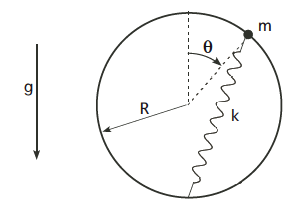
\includegraphics[scale=0.8]{Graphics/h5p3}
\end{center}

(a) What is the speed v of the bead when $\theta = \ang{90}$? Express your answer in terms of $m$, $R$, $k$, and $g$.\\
(b) What is the magnitude of the force the hoop exerts on the bead when $\theta = \ang{90}$? Express your answer in terms of $m$, $R$, $k$, and $g$.''

Alright, let's start by identifying the forces on the bead. Gravity and spring forces are quite obvious, but is there anything else? Yes, there is: a normal force by the hoop itself -- which they ask for in part (b).

The centripetal force required for this motion is still $m \frac{v^2}{R}$ at all times, but $v$ is not a constant in this problem (since both gravity and the spring will change the bead's speed), so the centripetal force will vary, too.





Since there is no friction, and gravitational forces and spring forces are both conservative, let's try conservation of energy.

The initial energy is all either gravitational potential energy or and spring potential energy. Let's set $U_g = 0$ at the center of the circle; in that case, the initial gravitational potential energy is $m g R$, and the final, at $\theta = \ang{90}$ is $0$ by our definition.\\
There is no initial kinetic energy, since the initial speed was negligible.\\
What about the spring? It is stretched a distance $R$ beyond its natural length (total length $2 R$,  natural length $R$) so it stores a potential energy $U_s = \frac{1}{2} k R^2$ at the top.

\begin{equation}
E = m g R + \frac{1}{2} k R^2
\end{equation}

At $\theta = \ang{90}$, all gravitational potential energy, and part of the spring's, will have turned into kinetic energy in the bead.

Here, the kinetic energy is $\frac{1}{2} m v^2$. The spring's stored energy is related to how far it is stretched beyond $R$; how far is that, at this point?\\
If we draw this up, with a $\theta$ as a right angle, and we draw a triangle with the spring length as the hypotenuse, the left and top sides of the triangle are both $R$ in length, so the hypotenuse (the spring's current length) is $x = \sqrt{2 R^2} = \sqrt{2} \times R$.
It is then stretched $d = R \sqrt{2} - R = R(\sqrt{2} - 1)$ beyond its natural length. That gives it a potential energy of $U_s = \frac{1}{2} k R^2(2 - 2 \sqrt{2} + 1)$.

Adding it all up, and setting it equal to $E$ above, which is the total energy at all times:

\begin{align}
\frac{1}{2} m v^2 + \frac{1}{2} k R^2(2 - 2 \sqrt{2} + 1) = m g R + \frac{1}{2} k R^2\\
m v^2 = 2 m g R + k R^2 - k R^2(2 - 2 \sqrt{2} + 1)\\
m v^2 = 2 m g R + k R^2 (1 - (2 - 2 \sqrt{2} + 1))\\
m v^2 = 2 m g R + k R^2 (-2 + 2 \sqrt{2})\\
v = \sqrt{\frac{2 m g R + k R^2 (-2 + 2 \sqrt{2})}{m}}
\end{align}

Next, we need to find the magnitude of the normal force from the hoop on the bead.

The \emph{radial} force (inwards) must always add up to the centripetal force, so we can decompose the forces and set that equal to $\frac{m v^2}{R}$.

Gravity at $\theta = \ang{90}$ is clearly purely tangential; there's no left-or-right force due to gravity. In other words, we can ignore gravity for this part.

The spring force, on the other hand, clearly has components both tangential (up/down) and radial (left/right) at this point.\\
The total spring force is proportional to its extension past $R$ (its natural length), which we found earlier, so

\begin{equation}
F_{spr} = k (\sqrt{2 R^2} - R) = k \sqrt{2} R - k R = k R (\sqrt{2} - 1)
\end{equation}

The above is the total spring force; we only want the radial component, which is $1/\sqrt{2}$ times that, or $F_{spr,rad} = k R(1 - 1/\sqrt{2})$.

The normal force is then the centripetal force $\frac{m v^2}{R}$, minus the force in that direction that the spring provides. (That is, the hoop must provide all the necessary force that the spring isn't.)

\begin{align}
N + k R(1 - \frac{1}{\sqrt{2}}) &= \frac{m v^2}{R}\\
N + k R(1 - \frac{1}{\sqrt{2}}) &= 2 m g + k R(2\sqrt{2} - 2)
\end{align}
\begin{align}
N &= 2 m g + k R\left(2\sqrt{2} - 2 - 1 + \frac{1}{\sqrt{2}}\right)\\
N &= 2 m g + k R\left(\frac{5}{\sqrt{2}} - 3\right)
\end{align}

That's it!

\section{Problem 4: Moon}

``A planet has a single moon that is solely influenced by the gravitational interaction between the two bodies. We will assume that the moon is moving in a circular orbit around the planet and that the moon travels with a constant speed in that orbit. The mass of the planet is $m_p = \SI{3.03e25}{kg}$. The mass of the moon is $m_m = \SI{9.65e22}{kg}$. The radius of the orbit is $R = \SI{2.75e8}{m}$.

What is the period of the moon's orbit around the planet in earth days (1 earth day = 24 hours).''

The moon is about 300 times more massive than the planet; I will assume that makes it valid to use the formulas we've already used (that are not valid if the masses are close to each other; more on that and center on mass very soon -- in the next problem).

As with the previous problem regarding orbit, I will use $E = \frac{1}{2} U$ here -- it's easy to remember, so why not?

\begin{align}
K_E + U &= \frac{1}{2} U\\
K_E + \frac{1}{2} U &= 0\\
\frac{1}{2} m_m v_{orbit}^2 - \frac{1}{2} \frac{G m_p m_m}{R} &= 0\\
v_{orbit}^2 - \frac{G m_p}{R} &= 0\\
v_{orbit} &= \sqrt{\frac{G m_p}{R}}
\end{align}

The period is then simply the distance divided by the velocity:

\begin{align}
T &= \frac{2 \pi R}{v_{orbit}} = 2 \pi R \sqrt{\frac{R}{G m_p}}\\
T &= 2 \pi \sqrt{\frac{R^3}{G m_p}} = 2 \pi \frac{R^{3/2}}{\sqrt{G m_p}} \approx \SI{637374}{s}
\end{align}

Finally, we just need to divide this by one ``Earth day'' of 86400 seconds, so the answer is $637374/86400 \approx 7.38$ days.

\section{Problem 5: Double star system}

``Consider a double star system under the influence of the gravitational force between the stars. Star 1 has mass $m_1 = \SI{2.22e31}{kg}$ and Star 2 has mass $m_2 = \SI{1.64e31}{kg}$. Assume that each star undergoes uniform circular motion about the center of mass of the system (cm). In the figure below $r_1$ is the distance between Star 1 and cm, and $r_2$ is the distance between Star 2 and cm.''

\begin{center}
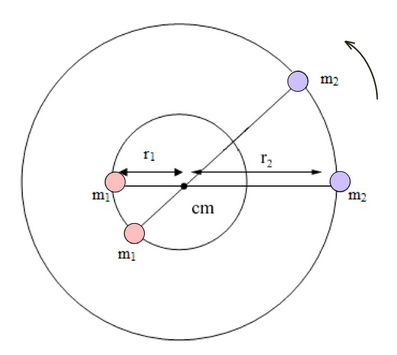
\includegraphics[scale=0.65]{Graphics/h5p5}
\end{center}

Ah, this week's possibly-scary problem. The concept of \emph{center of mass} should make it easy, though, especially since the period is the same for both stars.

The center of mass of a system is a point around which \emph{both} stars orbit. (In our solar system, the center of mass is inside the Sun, since it's such a dominant mass, but it's not at the Sun's center -- so the Sun actually makes a tiny orbit around the center of mass).

Apparently, in the case of two bodies, $m_1 r_1 = m_2 r_2$ will hold. Combined with $s = r_1 + r_2$ where $s$ is a given, we already have two equations and two unknowns. Too easy.

We can solve the second equation to give $r_1 = s - r_2$ and substitute into the first, to give one equation with one unknown:

\begin{align}
m_1 (s - r_2) &= m_2 r_2\\
m_1 r_2 +m_2 r_2 &= m_1 s\\
r_2(m_1 + m_2) &= m_1 s
\end{align}
\begin{equation}
r_2 = \frac{m_1 s}{m_1 + m_2}
\end{equation}

We can then find $r_2$ easily, and $r_1 = s - r_2$ as mentioned, so that too is easy. For the given values,

\begin{align}
r_1 = \SI{1.411e18}{m}\\
r_2 = \SI{1.909e18}{m}
\end{align}

Now, we just need to find the period. If the bodies orbit as shown, the gravitational attraction between them is always towards the center of mass. We can find $\omega$ this way, by equating the centripetal force $m |a_c| = m \omega^2 r$ with the gravitational force on one of the masses:

\begin{align}
m_1 \omega^2 r_1 &= \frac{G m_1 m_2}{s^2}\\
\omega^2 &= \frac{G m_1 m_2}{m_1 r_1 s^2}\\
\omega &= \sqrt{\frac{G m_2}{r_1 s^2}}
\end{align}

Finally, $\displaystyle T = \frac{2 \pi}{\omega}$:

\begin{align}
T &= 2 \pi \sqrt{\frac{r_1 s^2}{G m_2}} \approx \SI{7.505e17}{s} \approx \SI{23.8}{billion years}
\end{align}

This is, incredibly enough, correct. The staff admitted in a forum post that the value for the distances was way, way larger than what is realistic (by 6 orders of magnitude), and so the period grew to about $10^9$ times larger than expected!

\section{Problem 6: Potential energy diagram}

``A body of mass $m = 1$ kg is moving along the x-axis. Its potential energy is given by the function

\begin{equation*}
U(x) = 2 (x^2 - 1)^2
\end{equation*}

Note: The units were dropped for the numbers in the equation above. You should note that 2 would carry units of $\text{J} \cdot \text{m}^{-4}$ and 1 would carry units of $\text{m}^2$.

\begin{center}
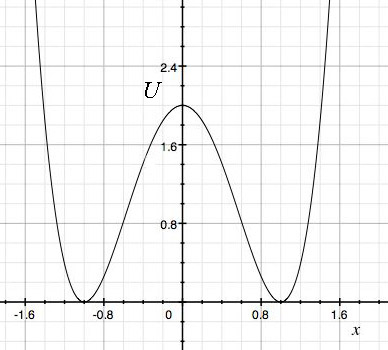
\includegraphics[scale=0.75]{Graphics/h5p6}
\end{center}

a) What is the $x$ component of the force associated with the potential energy given by $U(x)$? Give an expression in terms of $x$.\\
b) At what positive value of $x$ ($x > 0$) in m, does the potential have a stable equilibrium point?\\
c) Suppose the body starts with zero speed at $x = 1.5$ m. What is its speed (in m/s) at $x = 0$ m and at $x = -1$ m?''

Well, (b) is easy from the graph -- it is at $x = 1$. But let's avoid getting ahead of ourselves.

The important thing to remember here is that $\displaystyle \frac{dU}{dx} = - F_x$. So far part (a), we need to find the derivative of $U(x)$, and then remember to negate the answer. Using the chain rule,

\begin{align}
\frac{dU}{dx} &= 4(x^2 - 1)(2x) = 4(2x^3 - 2x) = 8x^3 - 8x\\
F_x = - \frac{dU}{dx} &= 8x - 8x^3 = 8(x - x^3)
\end{align}

For a more rigorous solution of part (b), we can find where $F_x = 0$, and only look at the cases where $x > 0$, which is the condition given:

\begin{align}
8(x - x^3) &= 0\\
x^3 &= x\\
x^2 &= 1\\
x &= \pm \sqrt{1}
\end{align}

For $x > 0$, the only solution is $x = 1$. As a last step, we can confirm whether this is a stable equilibrium point, or an unstable one. It's clear from the graph that it's stable (if there is a small amount of force on the body, it will tend to roll back down from the ``hills'', rather than roll away, as it would from one of the peaks).

Mathematically, the condition here is that the second derivative of $U$ is positive; that makes the curve ``concave upward'', i.e. looks like a U shape, so that things tend to stay inside. If $\displaystyle \frac{d^2U}{dx^2} < 0$, the opposite is true, and we are at a peak.

We calculate the second derivative, and stick $x = 1$ in there:

\begin{align}
24x^2 - 8 \overset{?}{>} 0\\
16 > 0
\end{align}

The second derivative is positive, and so this is indeed a \emph{stable} equilibrium point. If we try this at $x = 0$, we find $-8$, less than zero, and indeed, that is an unstable equilibrium point according to the graph.

Next, part (c), which asked

``c) Suppose the body starts with zero speed at $x = 1.5$ m. What is its speed (in m/s) at $x = 0$ m and at $x = -1$ m?''

Okay, so what does this imply? It starts at rest (zero kinetic energy), and we can easily calculate $U(1.5)$. We can then easily calculate $U(0)$, subtract the two, and we know the change in kinetic energy, and can solve for $v$.

\begin{align}
K_E(0) = U(1.5) - U(0)\\
\frac{1}{2} m v^2 = 2(1.5^2 - 1)^2 - 2(-1)^2\\
\frac{1}{2} m v^2 = 3.125 - 2 = 1.125\\
v = \sqrt{2.25} = \SI{1.5}{m/s}
\end{align}

For $x = -1$, we simply do the same thing, but use $U(-1)$ instead of $U(0)$.

\begin{align}
K_E(0) = U(1.5) - U(-1)\\
\frac{1}{2} m v^2 = 3.125\\
v = \sqrt{6.25} = \SI{2.5}{m/s}
\end{align}

\section{Problem 7: Earth drilling}

``A hole is drilled with smooth sides straight through the center of the earth to the other side of the earth. The air is removed from this tube (and the tube doesn't fill up with water, liquid rock or iron from the core). An object is dropped into one end of the tube and just reaches the opposite end. You can assume the earth is of uniform mass density. You can neglect the amount of mass drilled out and the rotation of the earth.

\begin{center}
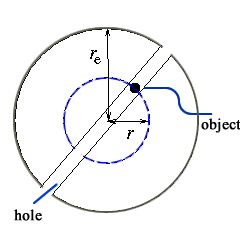
\includegraphics[scale=0.75]{Graphics/h5p7}
\end{center}

(a) The gravitational force on an object of mass $m$ located inside the earth a distance $r < r_e$ from the center ($r_e$ is the radius of the earth) is due only to the mass of the earth that lies within a solid sphere of radius $r$. What is the magnitude of the gravitational force as a function of the distance $r$ from the center of the earth? Express your answer in terms of the gravitational of the $r$, $m$, $g$, and $r_e$.

Note: you do not need the mass of the earth $m_e$ or the universal gravitation constant $G$ to answer this question but you will need to find an expression relating $m_e$ and $G$ to $g$ and $r_e$.''

Ah, I actually solved this on the forum last week or so, using Gauss's law. I will try to do it this way instead, here, though.

At the surface,

\begin{equation}
F_g = m g = \frac{G m m_e}{r_e^2}
\end{equation}

The fraction of Earth's mass inside this smaller radius $r$ is just the ratio of the volume of $r$ to the volume of $r_e$. I will call this mass $m_r$, so

\begin{align}
m_r &= \frac{4/3 \pi r^3}{4/3 \pi r_e^3} m_e\\
m_r &= \frac{r^3}{r_e^3} m_e
\end{align}

\begin{align}
F_i &= \frac{G m}{r^2} \frac{r^3}{r_e^3} m_e\\
F_i &= \frac{G m r}{r_e^3} m_e
\end{align}

Almost there... we need to get rid of that $G$, and write it in terms of $g$ instead. We have an equation for $F_g = m g$ in terms of $G$ and so on above, so we solve that one for $G$, and substitute in in here:

\begin{equation}
G = \frac{g r_e^2}{m_e}
\end{equation}

\begin{align}
F_i &= \frac{m r}{r_e^3} m_e \left(\frac{g r_e^2}{m_e}\right)\\
F_i &= \frac{m g r}{r_e}
\end{align}

Got it!

Next, part (b): ``How long would it take for this object to reach the other side of the earth? Express your answer in terms of the gravitational constant at the surface of earth $g$, $m$, and $r_e$ as needed.''

Okay, so the force experienced by the mass, at all times, is the force shown above. We can find the acceleration simply by dividing out $m$. If the acceleration were constant, we could use a simple kinematics equation here... but it's not constant. The velocity will not be constant, either, so we can't simply find a value for the velocity and calculate the time from knowing distance and velocity.

However...! The force is in the form $F = k r$, where $k = \frac{m g}{r_e}$ is a \emph{constant}, in newtons per meter. In other words, this looks like a spring problem, in a way. Not exactly, perhaps, but close enough: consider a spring of near-zero natural length, attached at the center of the Earth. It will always have an inwards force, which is proportional to $r$, the distance you've stretched it beyond its original zero length.

Once you've passed the center, it will still be an inwards force, that is now trying to make you stop and reverse. One full oscillation of this system will then bring you all the way to the other side, and then back, in a symmetric motion. Therefore, the answer is half the period.

\begin{equation}
T = \frac{2 \pi}{\omega} = 2\pi \sqrt{\frac{m}{k}} = 2\pi \sqrt{\frac{m}{mg/r_e}} = 2 \pi \sqrt{\frac{r_e}{g}}
\end{equation}

Half this is then simply

\begin{equation}
\frac{T}{2} = \pi\sqrt{\frac{r_e}{g}}
\end{equation}

\end{document}